\documentclass[12pt]{article}
\usepackage[latin1,utf8x]{inputenc}
\usepackage[spanish]{babel}
\usepackage{amsmath}
\usepackage{amsthm}
\usepackage{graphicx}
\usepackage{tabularx}
\usepackage{float}
\usepackage{anysize}
\numberwithin{equation}{section}
\marginsize{1.5cm}{1.5cm}{0cm}{2cm}
\author{M. en C. Gustavo Contreras Mayén.}
\title{Ejemplo con una ecuación diferencial parcial elíptica \\ \begin{Large}Curso de Fí­sica Computacional\end{Large}}
\date{ }
\begin{document}
\maketitle
De acuerdo a la que vimos en clase, tenemos el siguiente problema para la ecuación de Poisson:
\begin{figure} [!h]
	\centering
	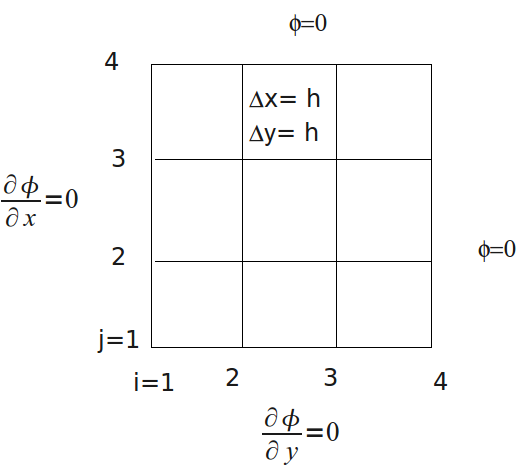
\includegraphics[scale=0.4]{Ejemplo1.png} 
	\caption{Malla para el problema.}
	\label{fig:malla1}
\end{figure}
\begin{enumerate}
\item Escribe la aproximación por diferencias de la ecuación de Poisson, para la retícula que se muestra en la figura \ref{fig:malla1}.
\\
Dado que la malla tiene una separación uniforme en ambas direcciones, las ecuaciones en diferencias se pueden escribir como:
\begin{eqnarray*}
	4 \phi_{1,1} - 2 \phi_{2,1} - 2 \phi_{1,2} & = & h^{2}S_{1,1} \\
	4 \phi_{2,1} - \phi_{1,1} - \phi_{3,1} - 2 \phi_{2,2} & = & h^{2}S_{2,1} \\			4 \phi_{3,1} - \phi_{2,1} - 2 \phi_{3,2} & = & h^{2}S_{3,1} \\
	4 \phi_{1,2} - 2 \phi_{2,2} - \phi_{1,2} - \phi_{1,3} & = & h^{2}S_{1,2} \\
	4 \phi_{2,2} - \phi_{1,2} - \phi_{3,2} - \phi_{2,1}  & = & h^{2}S_{2,2} \\
	4 \phi_{3,2} - \phi_{2,2} - \phi_{3,1} - \phi_{3,3}  & = & h^{2}S_{3,2} \\
	4 \phi_{1,3} - 2 \phi_{2,3} - \phi_{1,2} & = & h^{2}S_{1,3} \\
	4 \phi_{2,3} - \phi_{1,3} - \phi_{3,3} - \phi_{2,2}  & = & h^{2}S_{2,3} \\
	4 \phi_{3,3} - \phi_{3,2} - \phi_{2,3} & = & h^{2}S_{3,3} \\
\end{eqnarray*}
donde se usó que $\phi_{4,1}=\phi_{4,2}=\phi_{4,3}=\phi_{4,4}=\phi_{1,4}=\phi_{2,4}=\phi_{3,4}=0$.
\item En notacion matricial, las ecuaciones anteriores se escribirían de la siguiente manera:
\begin{equation*}
	\begin{pmatrix}
		4 & -2 & 0 & -2 & 0 & 0 & 0 & 0 & 0 \\
		-1 & 4 & -1 & 0 & -2 & 0 & 0 & 0 & 0 \\
		0 & -1 & 4 & 0 & 0 & -2 & 0 & 0 & 0 \\
		-1 & 0 & 0 & 4 & -2 & 0 & -1 & 0 & 0 \\
		0 & -1 & 0 & -1 & 4 & -1 & 0 & -1 & 0 \\
		0 & 0 & -1 & 0 & -1 & 4 & 0 & 0 & -1 \\
		0 & 0 & 0 & -1 & 0  & 0 & 4 & -2 & 0 \\
		0 & 0 & 0 & 0 & -1 & 0 & -1 & 4 & -1 \\
		0 & 0 & 0 & 0 & 0 & -1 & 0 & -1 & 4 	
	\end{pmatrix}
	\begin{pmatrix}
		\phi_{1,1} \\
		\phi_{2,1} \\
		\phi_{3,1} \\
		\phi_{1,2} \\
		\phi_{2,2} \\
		\phi_{3,2} \\
		\phi_{1,3} \\
		\phi_{2,1} \\
		\phi_{3,3} 
	\end{pmatrix}
		=
	\begin{pmatrix}
		h^{2} S_{1,1} \\
		h^{2} S_{2,1} \\
		h^{2} S_{3,1} \\
		h^{2} S_{1,2} \\
		h^{2} S_{2,2} \\
		h^{2} S_{3,2} \\
		h^{2} S_{1,3} \\
		h^{2} S_{2,3} \\
		h^{2} S_{3,3}
	\end{pmatrix}
\end{equation*}
\item La matriz de coeficientes se puede transformar en una forma simétrica al dividir entre 4 la primera ecuación  y dividiendo entre 2 también las ecuaciones segunda, tercera, cuarta y séptima:
\begin{equation*}
	\begin{pmatrix}
	1 & - \frac{1}{2} & 0 & - \frac{1}{2} & 0 & 0 & 0 & 0 & 0 \\
	- \frac{1}{2} & 2 & - \frac{1}{2} & 0 & -1 & 0 & 0 & 0 & 0 \\
	0 & -\frac{1}{2} & 2 & 0 & 0 & -1 & 0 & 0 & 0 \\
	- \frac{1}{2} & 0 & 0 & 2 & -1 & 0 & - \frac{1}{2} & 0 & 0 \\
	0 & -1 & 0 & -1 & 4 & -1 & 0 & -1 & 0 \\
	0 & 0 & -1 & 0 & -1 & 4 & 0 & 0 & -1 \\
	0 & 0 & 0 & - \frac{1}{2} & 0 & 0 & 2 & -1 & 0 \\
	0 & 0 & 0 & 0 & -1 & 0 & -1 & 4 & -1 \\
	0 & 0 & 0 & 0 & 0 & -1 & 0 & -1 & 4 
	\end{pmatrix}
	\begin{pmatrix}
		\phi_{1,1} \\
		\phi_{2,1} \\
		\phi_{3,1} \\
		\phi_{1,2} \\
		\phi_{2,2} \\
		\phi_{3,2} \\
		\phi_{1,3} \\
		\phi_{2,1} \\
		\phi_{3,3} 
	\end{pmatrix}
		=
	\begin{pmatrix}
		h^{2} S_{1,1} \\
		h^{2} S_{2,1} \\
		h^{2} S_{3,1} \\
		h^{2} S_{1,2} \\
		h^{2} S_{2,2} \\
		h^{2} S_{3,2} \\
		h^{2} S_{1,3} \\
		h^{2} S_{2,3} \\
		h^{2} S_{3,3}
	\end{pmatrix}
\end{equation*}
\textit{Nota: } como lo muestra el último arreglo matricial, la matriz de coeficientes de las ecuaciones en diferencias para el caso de la ecuación de Poisson sobre una malla rectangular tiene las siguientes propiedades:
\begin{enumerate}
\item la matriz es tridiagonal por bloques.
\item los bloques diagonales son submatrices diagonales.
\item los bloques fuera de la diagonal, pero adyacentes a los bloques en la digaonal, son submatrices cuyos elementos sobre la diagonal son negativos.
\item los demás bloques son submatrices nulas.
\item la matriz completa es simétrica.
\end{enumerate}
El número de elementos nulos crece rápidamente junto con el número total de puntos de la retícula. Si el espacio de memoria de la máquina es limitado, los métodos de solución iterativa son útiles en el caso de EDO elípticas, puesto que almacenan sólo los elementos no nulos de la matriz, de forma que se necesita mucho menos espacio de memoria que el método de solución directa.
\end{enumerate}
\end{document}